\chapter{Galois Representations, Reciprocity and Functoriality}\label{ch:03}

In 1880 Frobenius observed that the way a prime $p$ factors in a Galois extension is governed by a single conjugacy class in the Galois group, and he conjectured that every class occurs with a frequency proportional to its size. Chebotarev proved the conjecture in 1922; his proof appeared in Russian in 1923 and in German in 1926. Read with a probabilist's eye, his theorem says that the Frobenius class of a random prime is distributed as the conjugacy class of a uniformly random element of a finite group. Much of this book elaborates that sentence, replacing the finite group by a compact Lie group. This chapter assembles the arithmetic objects involved: Galois representations, reciprocity, the dual group and the Satake isomorphism, functoriality, and the Sato Tate group. We prove nothing new about reciprocity or functoriality; our purpose is to state the conjectures precisely, to say which cases are proved, and to isolate the probabilistic statements they imply.

\section{Frobenius elements and the Chebotarev density theorem}\label{sec:ch3cheb}

The absolute Galois group\index{absolute Galois group} $G_\Q=\Gal(\overline{\Q}/\Q)$ is the inverse limit of $\Gal(L/\Q)$ over finite Galois extensions $L$. Let $L/\Q$ be finite Galois with group $G$ and absolute discriminant $d_L$, and let $p$ be unramified in $L$, that is, $p\nmid d_L$. Choose a prime $\mathfrak{P}$ of $L$ above $p$, with residue field $\mathbb{F}_{\mathfrak{P}}$. Since the inertia group of $\mathfrak{P}$ is trivial, the decomposition group $\{\sigma\in G:\sigma\mathfrak{P}=\mathfrak{P}\}$ maps isomorphically onto $\Gal(\mathbb{F}_{\mathfrak{P}}/\mathbb{F}_p)$, which is generated by $t\mapsto t^p$, and the preimage of this generator is the Frobenius element\index{Frobenius element} $\Frob_{\mathfrak{P}}\in G$, characterised by
\[
\Frob_{\mathfrak{P}}(\alpha)\equiv\alpha^p \pmod{\mathfrak{P}}\qquad\text{for all algebraic integers }\alpha\in L .
\]
Changing $\mathfrak{P}$ to $\sigma\mathfrak{P}$ conjugates $\Frob_{\mathfrak{P}}$ by $\sigma$, so $p$ determines a conjugacy class $\Frob_p\subset G$. For a representation $\rho$ of $G_\Q$ unramified at $p$, that is, trivial on the inertia groups of the primes above $p$, the matrix $\rho(\Frob_p)$ is therefore defined up to conjugacy, and its trace and characteristic polynomial are well defined. If $L$ is the splitting field of a monic irreducible $f\in\Z[x]$ and $p\nmid\operatorname{disc}(f)$, the cycle type of $\Frob_p$ on the roots is the list of degrees of the irreducible factors of $f$ modulo $p$ (Dedekind).

\begin{theorem}[Chebotarev density theorem]\label{thm:ch3cheb}
Let $L/\Q$ be a finite Galois extension with group $G$ and let $C\subset G$ be a conjugacy class. Then
\[
\lim_{x\to\infty}\frac{\#\{p\le x:\ p\text{ unramified in }L,\ \Frob_p=C\}}{\pi(x)}=\frac{|C|}{|G|}.
\]
\end{theorem}

The theorem is due to Chebotarev \cite{chebotarev1926}. Effective forms are due to Lagarias and Odlyzko \cite{lagariasodlyzko1977}: under the generalized Riemann hypothesis for the Dedekind zeta function of $L$, the count in the numerator is $(|C|/|G|)\operatorname{Li}(x)$ up to an error $O\bigl((|C|/|G|)\sqrt x\log(d_Lx^{[L:\Q]})+\log d_L\bigr)$, with an absolute implied constant, where $\operatorname{Li}(x)=\int_2^x dt/\log t$. Serre \cite{serre1981} develops applications.\index{Chebotarev density theorem}

\begin{corollary}[Chebotarev as equidistribution]\label{cor:ch3cheb}
Let $h$ be the uniform probability measure on $G$. For every class function $\phi:G\to\C$,
\[
\frac{1}{\pi(x)}\sum_{p\le x,\ p\nmid d_L}\phi(\Frob_p)\longrightarrow\int_G\phi\,dh .
\]
Equivalently, if $P$ is chosen uniformly from the unramified primes up to $x$, then the class $\Frob_P$ converges in law, as $x\to\infty$, to the conjugacy class of a uniformly random element of $G$.
\end{corollary}

\begin{proof}
Indicators of conjugacy classes span the class functions, and $h(C)=|C|/|G|$. Ramified primes are finite in number.
\end{proof}

Since irreducible characters span the class functions, Corollary~\ref{cor:ch3cheb} is equivalent to $\pi(x)^{-1}\sum_{p\le x,\,p\nmid d_L}\chi(\Frob_p)\to0$ for every nontrivial irreducible character $\chi$ of $G$. This is the finite group case of the Weyl criterion (Theorem~\ref{thm:04weyl}), and it gives a modern proof: the limit follows by a Tauberian argument from the holomorphy and nonvanishing on $\Re s\ge1$ of the Artin $L$ functions of Section~\ref{sec:ch3artin}. Chebotarev's own proof reduced the theorem to abelian extensions by adjoining roots of unity.

\begin{example}[The cubic $x^3-x-1$]\label{ex:ch3cubic}
Let $f=x^3-x-1$, with discriminant $-23$. Its splitting field $L$ has group $S_3$ and is the Hilbert class field of $\Q(\sqrt{-23})$, which has class number $3$. For $p\ne23$ the identity class has size $1$ ($f$ splits into linear factors), the transpositions have size $3$ ($f$ has exactly one root modulo $p$), and the $3$ cycles have size $2$ ($f$ is irreducible modulo $p$). Chebotarev predicts frequencies $1/6$, $1/2$, $1/3$. We computed the class of $\Frob_p$ for all $664{,}578$ primes $p<10^7$ with $p\ne23$, using the Kronecker symbol $(-23/p)$ and a test of $x^p\equiv x$ in $\mathbb{F}_p[x]/(f)$. The observed frequencies are
\[
0.16637,\qquad 0.50027,\qquad 0.33336,
\]
against $0.16667$, $0.5$, $0.33333$; Figure~\ref{fig:ch03_chebotarev} shows the convergence. The two dimensional irreducible representation $\rho$ of $S_3$ has character values $2,0,-1$ on the three classes. It is induced from a character of order $3$ of the class group of $\Q(\sqrt{-23})$, so Hecke's theory of theta series shows that the numbers $\tr\rho(\Frob_p)$, $p\ne23$, are the Fourier coefficients at primes of a weight one cusp form of level $23$, namely $\eta(z)\eta(23z)$. This classical nonabelian instance of reciprocity reappears in Chapter~\ref{ch:recip} as the main test case of its reciprocity criteria, in Chapter~\ref{ch:11} as an extreme value law, and in Chapter~\ref{ch:flt}, through Wilton's congruence for $\tau(p)$ modulo $23$, as the prototype of the congruences between forms of weight one and of higher weight used in the proof of Fermat's last theorem. In Chapter~\ref{ch:lap} the Frobenius traces are read off the transported density of $\eta(z)\eta(23z)$, and the form is rebuilt from the Artin $L$ function by Bromwich inversion on the critical line, which uses the holomorphy that Hecke's theorem supplies.
\end{example}

\begin{figure}[t]\centering
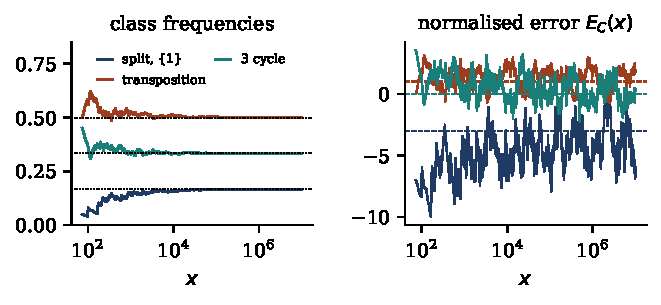
\includegraphics[width=\textwidth]{figs/ch03_chebotarev.pdf}
\caption{Chebotarev for $x^3-x-1$, with Galois group $G=S_3$, primes below $10^7$. Left: frequencies of the three Frobenius classes (split completely, transposition, $3$ cycle) among the unramified primes up to $x$, against $1/6,1/2,1/3$. Right: the normalised error $E_C(x)=(\log x/\sqrt x)\,(|G|\pi_C(x)/|C|-\pi^{\mathrm{ur}}(x))$, where $\pi_C(x)$ and $\pi^{\mathrm{ur}}(x)$ count the unramified primes $p\le x$ with $\Frob_p=C$ and in total; dashed lines mark the limiting means $1-r_C/|C|=-3,1,0$ produced by the prime squares, where $r_C=\#\{g\in G:g^2\in C\}$.}\label{fig:ch03_chebotarev}
\end{figure}

The right panel shows a second order effect. Write $\pi_C(x)$ for the number of unramified $p\le x$ with $\Frob_p=C$, $\pi^{\mathrm{ur}}(x)=\sum_C\pi_C(x)$ for the number of unramified $p\le x$, and $E_C(x)=(\log x/\sqrt x)(|G|\pi_C(x)/|C|-\pi^{\mathrm{ur}}(x))$ for the normalised error. The prime squares enter the explicit formula through $\Frob_p^2$, distributed as $g^2$ for $g$ uniform in $G$. Under the Riemann hypothesis for the Artin $L$ functions of $L$, and since neither $L(s,\rho)$ nor the $L$ function of the sign character, which is the Dirichlet $L$ function of $(-23/\cdot)$, vanishes at $s=\frac12$, $E_C(x)$ is the constant $1-r_C/|C|$, up to $o(1)$, plus an oscillation driven by the zeros whose logarithmic mean is zero (Exercise~\ref{ex:ch3fs}). For $S_3$ the limiting means are $-3$, $1$ and $0$; our logarithmic averages over $10^3<x<10^7$ are $-4.3$, $1.2$ and $0.3$.

The gap is a lower order effect: the limits are approached only at the rate $1/\log x$. The explicit formula counts the prime powers $p^k$ with weight $1/k$, and $\pi_C(x)$ is what remains when the terms with $k\ge2$ are removed. Replacing the number of unramified primes $p\le y$ with $\Frob_p^k=C$ in those terms by its expected value $r_C^{(k)}\operatorname{li}(y)/|G|$ and the number of all unramified primes $p\le y$ by $\operatorname{li}(y)$, with $r_C^{(k)}=\#\{g\in G:g^k\in C\}$ (so $r_C=r_C^{(2)}$) and $\operatorname{li}(y)=\operatorname{Li}(y)+1.045\ldots$ the principal value logarithmic integral, adds $(\log x/\sqrt x)\sum_{k\ge2}k^{-1}(1-r_C^{(k)}/|C|)\operatorname{li}(x^{1/k})$ to $E_C(x)$, and the term $k=2$ equals $(1-r_C/|C|)(1+2/\log x+O(\log^{-2}x))$. The logarithmic means of this sum over $10^3<x<10^7$ are $-4.4$, $1.3$ and $0.2$ if only $k=2,3$ are kept, which is close to the observed values, but the truncation is arbitrary: keeping all $k$ with $2^k\le x$ gives $-5.0$, $1.5$ and $0.3$. The prime powers therefore explain the sign and the order of magnitude of the gap, not its exact value. The smallest primes are not spread over the classes as expected counts assume (the first prime that splits completely is $59$), and the remaining terms of the explicit formula oscillate with amplitude of order one and need not average out over a window of this length. Rubinstein and Sarnak \cite{rubinsteinsarnak1994} put Chebyshev's bias\index{Chebyshev bias} for primes in arithmetic progressions on a probabilistic footing, and their argument extends to Chebotarev classes: under the generalized Riemann hypothesis the law of $E_C(e^y)$, for $y$ uniform in $[0,Y]$, converges as $Y\to\infty$, and under a linear independence hypothesis on the zeros the limit is the law of the constant plus a weighted sum of independent uniformly distributed phases. In our data, primes that split completely are rarer than Chebotarev predicts, $6\pi_{\{1\}}(x)<\pi^{\mathrm{ur}}(x)$, for every $x$ with $2\le x<10^7$ outside $[2.02\times10^6,2.51\times10^6]$, and inside that interval except on short stretches of total length below $10^4$.

\section{Artin \texorpdfstring{$L$}{L} functions and \texorpdfstring{$\ell$}{l} adic representations}\label{sec:ch3artin}

Let $\rho:G_\Q\to\GL(V)$ be a continuous representation on a finite dimensional complex vector space, necessarily with finite image. Artin \cite{artin1924} defined
\[
L(s,\rho)=\prod_p\det\bigl(1-\rho(\Frob_p)p^{-s}\mid V^{I_p}\bigr)^{-1},
\]
where $I_p$ is an inertia group at $p$, $V^{I_p}$ is the subspace it fixes, and $\Frob_p$ acts on $V^{I_p}$ through any of its lifts; the product converges for $\Re s>1$. Brauer's induction theorem \cite{brauer1947} writes $L(s,\rho)$ as a product of integral powers of $L$ functions of one dimensional characters over intermediate fields, which class field theory identifies with Hecke $L$ functions. Hence $L(s,\rho)$ is meromorphic on $\C$ with a functional equation, and holomorphic and nonzero on $\Re s=1$ except for a pole at $s=1$ whose order is the multiplicity of the trivial representation in $\rho$. That is all that Chebotarev requires.\index{Artin $L$ function}

\begin{conjecture}[Artin]
If $\rho$ is irreducible and nontrivial, then $L(s,\rho)$ is entire.
\end{conjecture}

The Artin conjecture follows from reciprocity: if $\rho$ corresponds to a cuspidal automorphic representation of $\GL_n$, then $L(s,\rho)$ is entire by Godement and Jacquet \cite{godementjacquet1972}. For two dimensional $\rho$, odd or even, such a correspondence is known when the projective image is dihedral (Hecke), tetrahedral (Langlands \cite{langlands1980}) or octahedral (Langlands and Tunnell \cite{tunnell1981}). Every odd irreducible two dimensional $\rho$ comes from a weight one newform, by the proof of Serre's modularity conjecture by Khare and Wintenberger \cite{kharewintenberger2009,kharewintenberger2009b}, which also uses work of Kisin \cite{kisin2009}. The even icosahedral case is open, and in dimension three and higher the conjecture is open in general.

Geometry supplies representations with infinite image. For an elliptic curve $E/\Q$ and a prime $\ell$, the $\ell$ adic Tate module\index{Tate module} $T_\ell E=\varprojlim E[\ell^n]$, with $E[\ell^n]$ the $\ell^n$ torsion of $E(\overline{\Q})$, is free of rank $2$ over $\Z_\ell$ with a continuous action of $G_\Q$, giving $\rho_{E,\ell}:G_\Q\to\GL_2(\Z_\ell)$. It is unramified at every $p\nmid\ell N_E$, where $N_E$ is the conductor, and there
\[
\det\bigl(1-\rho_{E,\ell}(\Frob_p)T\bigr)=1-a_pT+pT^2,\qquad a_p=p+1-\#E(\mathbb{F}_p),
\]
independently of $\ell$; by Hasse the reciprocal roots have absolute value $\sqrt p$.

\begin{theorem}[Serre's open image theorem \cite{serre1972}]\label{thm:ch3serre}
Let $E/\Q$ be an elliptic curve without complex multiplication. Then $\rho_{E,\ell}(G_\Q)$ is open in $\GL_2(\Z_\ell)$ for every $\ell$, and equals $\GL_2(\Z_\ell)$ for all but finitely many $\ell$. The image of the adelic representation $G_\Q\to\GL_2(\widehat{\Z})$ is open.
\end{theorem}

Chebotarev, applied to the field cut out by $E[\ell^n]$, shows that the classes of $\rho_{E,\ell}(\Frob_p)\bmod\ell^n$ are equidistributed for the uniform measure on the image of $G_\Q$ in $\GL_2(\Z/\ell^n\Z)$. Hence, when $E$ has no complex multiplication, for all but finitely many $\ell$ and every $d\in\mathbb{F}_\ell^\times$, the residues $a_p\bmod\ell$ over primes $p\equiv d\bmod\ell$ are distributed as the trace of a uniform element of $\GL_2(\mathbb{F}_\ell)$ with determinant $d$. These congruence laws are the correction factors in the Lang and Trotter heuristic of Chapter~\ref{ch:05}. They say nothing about the archimedean size of $a_p/\sqrt p$; that is the content of Sato Tate, and its only known proof goes through automorphy.

The family $(\rho_{E,\ell})_\ell$ is the model of a compatible system\index{compatible system}: representations $\rho_\ell:G_\Q\to\GL_n(\overline{\Q}_\ell)$, one for each prime $\ell$, unramified outside $S\cup\{\ell\}$ for a fixed finite set $S$, such that for each $p\notin S$ the characteristic polynomial of $\rho_\ell(\Frob_p)$, $\ell\ne p$, has coefficients in a fixed number field embedded in every $\overline{\Q}_\ell$ and does not depend on $\ell$. The cohomology $H^i_{\mathrm{et}}(X_{\overline{\Q}},\Q_\ell)$ of a smooth projective variety $X/\Q$ gives one, with $S$ the primes of bad reduction, and by Deligne \cite{deligne1974} for $p\notin S$ the eigenvalues of the geometric Frobenius $\rho_\ell(\Frob_p)^{-1}$ have absolute value $p^{i/2}$.

\section{Reciprocity}\label{sec:ch3recip}

The reciprocity conjecture of Langlands \cite{langlands1970} predicts that every irreducible compatible system arising from geometry corresponds to a cuspidal automorphic representation $\pi$ of $\GL_n(\A_\Q)$: for almost all $p$ the characteristic polynomial of $\rho_\ell(\Frob_p)$ is the Satake polynomial of $\pi_p$, suitably normalised. We record what is known for $n\le2$ over $\Q$ in the cases this book uses.\index{reciprocity}

\subsection{The case \texorpdfstring{$\GL_1$}{GL1}: class field theory}

A continuous character $G_\Q\to\C^\times$ has finite image, so by the Kronecker and Weber theorem it factors through $\Gal(\Q(\zeta_m)/\Q)\cong(\Z/m\Z)^\times$ for some $m$, and is a Dirichlet character. Over a number field $F$, global class field theory identifies the abelianisation of $G_F$ with the group of connected components of the idele class group $F^\times\backslash\A_F^\times$, so that characters of finite order of $G_F$ correspond to Hecke characters of finite order. Reciprocity for $\GL_1$ is a theorem.

\subsection{The case \texorpdfstring{$\GL_2$}{GL2} over \texorpdfstring{$\Q$}{Q}: modularity}

Let $f=\sum a_nq^n$ be a normalised cuspidal newform of weight $k\ge1$, level $N$ and nebentypus $\varepsilon$.

\begin{theorem}[Eichler, Shimura, Deligne, Deligne and Serre]\label{thm:ch3ES}
There is a number field $K_f$ containing the $a_n$, and for each prime $\lambda$ of $K_f$, of residue characteristic $\ell$, a continuous irreducible representation $\rho_{f,\lambda}:G_\Q\to\GL_2(K_{f,\lambda})$ unramified outside $N\ell$ with
\[
\tr\rho_{f,\lambda}(\Frob_p)=a_p,\qquad \det\rho_{f,\lambda}(\Frob_p)=\varepsilon(p)p^{k-1}\qquad(p\nmid N\ell).
\]
For $k=2$ this is due to Eichler \cite{eichler1954} and Shimura \cite{shimura1971}; for $k>2$ to Deligne \cite{deligne1971}, whose proof of the Weil conjectures \cite{deligne1974} then gives $|a_p|\le2p^{(k-1)/2}$; for $k=1$ to Deligne and Serre \cite{deligneserre1974}, who obtain an odd irreducible representation with finite image in $\GL_2(\C)$, unramified outside $N$. Irreducibility for $k\ge2$ is due to Ribet \cite{ribet1977}.
\end{theorem}

Conversely, by the modularity theorem (Theorem~\ref{thm:02modularity}) every elliptic curve $E/\Q$ arises from a newform $f$ of weight $2$ and level $N_E$, so that $L(s,E)=L(s,f)$.\index{modularity theorem} The proof is by modularity lifting, deformation theory matched against Hecke algebras; no probabilistic argument enters.

For the probabilist the Galois side gives congruences, with $\rho(\Frob_p)$ equidistributed in every finite quotient of the image; the automorphic side gives analysis, namely continuation and functional equations for symmetric powers and tensor products. Equidistribution of $a_p/p^{(k-1)/2}$ in $[-2,2]$ is proved through the second, which is why probability enters as a consequence of reciprocity and functoriality (Chapter~\ref{ch:01}).

\section{The dual group and the Satake isomorphism}\label{sec:ch3dual}

Let $G$ be a split connected reductive group over $\Q_p$, with split maximal torus $T$ and root datum $(X^*,\Phi,X_*,\Phi^\vee)$, where $X^*=X^*(T)$ and $X_*=X_*(T)$. The Langlands dual group\index{dual group} $\widehat G$ is the complex reductive group with the dual root datum $(X_*,\Phi^\vee,X^*,\Phi)$. Thus $\GL_n$ is self dual, $\SL_2$ and $\PGL_2$ are dual to each other, and $\mathrm{SO}_{2n+1}$ is dual to $\mathrm{Sp}_{2n}$. For a connected reductive group $G$ over a number field $F$, not necessarily split, the $L$ group is ${}^LG=\widehat G\rtimes W_F$, the Weil group $W_F$ acting through a finite quotient. Regard the split group $G$ as defined over $\Z_p$, let $K=G(\Z_p)$, and let $\mathcal{H}(G(\Q_p),K)$ be the spherical Hecke algebra of compactly supported $K$ biinvariant functions on $G(\Q_p)$ under convolution.

\begin{theorem}[Satake isomorphism \cite{satake1963}]\label{thm:ch3satake}
There is a canonical isomorphism of $\C$ algebras
\[
\mathcal{H}(G(\Q_p),K)\ \cong\ \C[X_*(T)]^{W}\ \cong\ \C[\widehat G]^{\widehat G},
\]
where $W$ is the Weyl group and the last algebra is the algebra of regular class functions on $\widehat G$, spanned by the characters of finite dimensional representations of $\widehat G$.
\end{theorem}

An irreducible smooth representation $\pi_p$ of $G(\Q_p)$ is unramified if it has a nonzero $K$ fixed vector. The space $\pi_p^K$ is then one dimensional, and $\mathcal{H}(G(\Q_p),K)$ acts on it by a character, which by Satake is evaluation at a semisimple conjugacy class $A(\pi_p)\subset\widehat G$, the Satake parameter\index{Satake parameter} of $\pi_p$. The map $\pi_p\mapsto A(\pi_p)$ is a bijection from isomorphism classes of unramified irreducible representations onto semisimple conjugacy classes in $\widehat G$; this is the unramified local Langlands correspondence. For $\GL_2$ and a newform $f$ of weight $k$ with $p\nmid N$, the unitarily normalised Satake parameter is the class of $\operatorname{diag}(\alpha_p,\beta_p)$ with $\alpha_p+\beta_p=a_p/p^{(k-1)/2}$ and $\alpha_p\beta_p=\varepsilon(p)$.

If $\pi_p$ is tempered, as Conjecture~\ref{conj:02ramanujan} predicts for the components of cuspidal representations of $\GL_n$ and as is known for holomorphic newforms, then $A(\pi_p)$ meets a maximal compact subgroup of $\widehat G$. The Hecke operator corresponding to the character $\chi_V$ of a representation $V$ of $\widehat G$ acts on $\pi_p^K$ by $\tr V(A(\pi_p))$. For $\GL_2$, a newform with trivial nebentypus and $V=\Sym^n$ this is $U_n(x_p/2)$ with $x_p=a_p/p^{(k-1)/2}$, the Chebyshev polynomial of the Weyl criterion for $\SU(2)$ in Chapter~\ref{ch:04}; with nontrivial nebentypus the identity fails (Exercise~\ref{ex:ch3neben}). After Satake, the spherical Hecke algebra is the complexified representation ring of the dual group. For $\PGL_2$, Chapter~\ref{ch:07} realises $T_p$ as the adjacency operator of the Bruhat Tits tree, $p+1$ times the transition operator of simple random walk.

\section{The principle of functoriality}\label{sec:ch3funct}

\begin{conjecture}[Functoriality; Langlands \cite{langlands1970}]\label{conj:ch3funct}
Let $G$ and $H$ be connected reductive groups over a number field $F$, with $G$ quasisplit, and let $r:{}^LH\to{}^LG$ be an $L$ homomorphism, that is, a continuous homomorphism compatible with the projections to $W_F$ and holomorphic on $\widehat H$. For every automorphic representation $\pi$ of $H(\A_F)$ there is an automorphic representation $\Pi$ of $G(\A_F)$ such that for almost all places $v$ the Satake parameter of $\Pi_v$ is $r(A(\pi_v))$.
\end{conjecture}

Here, at a finite place $v$ where $H$ and $\pi_v$ are unramified, $A(\pi_v)$ is the Satake parameter of $\pi_v$: a semisimple $\widehat H$ conjugacy class in the coset of ${}^LH$ above a Frobenius element of $W_{F_v}$ \cite{borel1979}, which is the class in $\widehat H$ of Section~\ref{sec:ch3dual} when $H$ is split; the same convention applies to $G$ and $\Pi_v$. The quasisplit hypothesis falls on the target: Jacquet and Langlands transfer from the multiplicative group of a quaternion algebra to $\GL_2$, but not every representation of $\GL_2$ transfers back. Taking $G=\GL_m$ and $r$ an $m$ dimensional representation of ${}^LH$, functoriality predicts that the automorphic $L$ function $L(s,\pi,r)$ is, up to finitely many Euler factors, a standard $L$ function of $\GL_m$, with continuation and a functional equation; see Arthur \cite{arthur2003} and Gelbart \cite{gelbart1984}. Here are the cases we use.\index{functoriality}

\begin{enumerate}
\item Symmetric powers. For $\pi$ on $\GL_2$ and $r=\Sym^n$, functoriality was proved for $n=2$ by Gelbart and Jacquet \cite{gelbartjacquet1978}, for $n=3$ by Kim and Shahidi \cite{kimshahidi2002}, and for $n=4$ by Kim \cite{kimsarnak2003}. Newton and Thorne \cite{newtonthorne2021,newtonthorne2021b} proved it for every $n$ when $\pi$ comes from a holomorphic newform of weight $k\ge2$ without complex multiplication. For Maass forms the cases $n\ge5$ are open.
\item Base change for $\GL_n$ along cyclic extensions of prime degree, and so along solvable Galois extensions by iteration, by Langlands \cite{langlands1980} for $n=2$ and Arthur and Clozel \cite{arthurclozel1989} for general $n$.
\item Jacquet Langlands. If $D$ is a quaternion algebra over $F$, Jacquet and Langlands \cite{jacquetlanglands1970} transferred automorphic representations of $D^\times(\A_F)$ of dimension greater than one to cuspidal representations of $\GL_2(\A_F)$, discrete series where $D$ ramifies. This identifies Hecke eigenvalues on the supersingular isogeny graphs of Chapter~\ref{ch:08} with Fourier coefficients of modular forms.
\item Tensor products. $\GL_2\times\GL_2\to\GL_4$ is functorial by Ramakrishnan \cite{ramakrishnan2000}, and $\GL_2\times\GL_3\to\GL_6$ by Kim and Shahidi \cite{kimshahidi2002}. The general case is open.
\end{enumerate}

The local Langlands correspondence\index{local Langlands correspondence} for $\GL_n$ over a finite extension $F_v$ of $\Q_p$ is a bijection from isomorphism classes of irreducible smooth representations of $\GL_n(F_v)$ to isomorphism classes of $n$ dimensional Frobenius semisimple Weil Deligne representations of $W_{F_v}$, characterised by local class field theory for $n=1$ and by compatibility with twists, central characters, duals and the $L$ and $\varepsilon$ factors of pairs. On unramified representations it is the bijection $\pi_p\mapsto A(\pi_p)$ of Section~\ref{sec:ch3dual}. It was proved by Harris and Taylor \cite{harristaylor2001} and by Henniart \cite{henniart2000}, with a later proof by Scholze \cite{scholze2013}.

\subsection{Potential automorphy and the Sato Tate theorem}

The Sato Tate theorem was proved before Newton and Thorne, from a weaker statement. A compatible system over a number field $F$ is potentially automorphic if its restriction to $G_{F'}$ is automorphic for some finite Galois extension $F'/F$; in the results quoted next, $F'$ can be chosen totally real when $F$ is. Clozel, Harris and Taylor \cite{cht2008}, Taylor \cite{taylor2008}, and Harris, Shepherd Barron and Taylor \cite{hsbt2010} proved potential automorphy of the odd symmetric powers $\Sym^{2m-1}\rho_{E,\ell}$ for elliptic curves over totally real fields with nonintegral $j$ invariant, which together with Rankin Selberg theory controls every symmetric power $L$ function. Barnet Lamb, Geraghty, Harris and Taylor \cite{blght2011} proved potential automorphy of all symmetric powers of holomorphic newforms of weight $k\ge2$ without complex multiplication, and noted that the hypothesis on the $j$ invariant can now be removed for elliptic curves without complex multiplication over totally real fields.

Potential automorphy suffices because Brauer's induction theorem, applied to $\Gal(F'/F)$, expresses $L(s,\Sym^n\rho)$ as a product of integral powers of $L$ functions over intermediate fields. The subgroups in Brauer's theorem are elementary, hence solvable, so solvable descent \cite{arthurclozel1989} makes these standard or Rankin Selberg $L$ functions of automorphic representations. Each is nonvanishing on $\Re s\ge1$ by the results of Jacquet and Shalika \cite{jacquetshalika1976} and Shahidi \cite{shahidi1981}, and holomorphic there except for the simple pole at $s=1$ of the Rankin Selberg factors $L(s,\pi\times\tilde\pi)$, which cancels in $L(s,\Sym^n\rho)$ for $n\ge1$. So $L(s,\Sym^n\rho)$ is meromorphic on $\C$, and holomorphic and nonzero on $\Re s\ge1$ for $n\ge1$, though not known from this argument to be entire. This is exactly the hypothesis of Serre's theorem (Theorem~\ref{thm:04serre}).

\begin{theorem}[Sato Tate; Clozel, Harris, Shepherd Barron, Taylor, Barnet Lamb, Geraghty]\label{thm:ch3ST}
Let $E/\Q$ be an elliptic curve without complex multiplication and, for $p\nmid N_E$, write $a_p=2\sqrt p\cos\theta_p$ with $\theta_p\in[0,\pi]$. Then $(\theta_p)$ is equidistributed with respect to $\frac2\pi\sin^2\theta\,d\theta$.
\end{theorem}

The proof is the archetype of the slogan that functoriality implies probability: potential automorphy gives the analysis of $L(s,\Sym^n E)$ for every irreducible representation $\Sym^n$ of $\SU(2)$, and the Weyl criterion converts it into a law of large numbers; Chapter~\ref{ch:04} gives the details. Harris~\cite{harris2009} proved the joint version, assuming results on Galois representations that were established soon afterwards: for two elliptic curves over a totally real field, without complex multiplication and not isogenous over an algebraic closure, the pairs $(\theta_p,\theta'_p)$ are equidistributed for the product of the two Sato Tate measures (over $\Q$ this is Theorem~\ref{thm:04joint}, where the hypotheses are discussed).

\section{The Sato Tate group}\label{sec:ch3stgroup}

Which compact group replaces $\SU(2)$ for a general motive? Serre gave the definition \cite{serre2012}, and Fité, Kedlaya, Rotger and Sutherland \cite{fkrs2012} showed that for abelian surfaces it is determined by the Galois module of endomorphisms. Let $A$ be an abelian variety of dimension $g$ over a number field $F$.\index{Sato Tate group}

\begin{definition}[Serre]\label{def:ch3stgroup}
Fix a prime $\ell$ and let $\rho_\ell:G_F\to\mathrm{GSp}_{2g}(\Q_\ell)$ be the action on $V_\ell A=T_\ell A\otimes\Q_\ell$, symplectic for the Weil pairing of a polarisation. Let $G_\ell$ be the Zariski closure of $\rho_\ell(G_F)$ in $\mathrm{GSp}_{2g}$, and $G^1_\ell=G_\ell\cap\mathrm{Sp}_{2g}$. Choose a field embedding $\iota:\Q_\ell\to\C$. The Sato Tate group $\mathrm{ST}(A)$ is a maximal compact subgroup of $G^1_\ell\otimes_\iota\C$, a compact subgroup of $\USp(2g)$ well defined up to conjugacy.
\end{definition}

For a prime $\mathfrak{p}\nmid\ell$ of $F$ at which $A$ has good reduction, with norm $N\mathfrak{p}$, the normalised Frobenius $\iota\rho_\ell(\Frob_{\mathfrak{p}})/\sqrt{N\mathfrak{p}}$ lies in $G^1_\ell(\C)$ and is semisimple with eigenvalues of absolute value one, so it defines a conjugacy class $s_{\mathfrak{p}}$ in $\mathrm{ST}(A)$. Independence of $\ell$ and $\iota$ is known for $g\le3$. Let $K$ be the smallest extension of $F$ over which all endomorphisms of $A$ are defined. Then $\Gal(K/F)$ is a quotient of the component group $\mathrm{ST}(A)/\mathrm{ST}(A)^0$, and the two are isomorphic when $g\le3$ \cite{banaszakkedlaya2015,fkrs2012,sutherland2019}, so that Chebotarev for $K/F$ governs which component contains $s_{\mathfrak{p}}$; for general $g$ the same role is played by the extension of $F$ cut out by the component group, which contains $K$.

\begin{conjecture}[Generalised Sato Tate]\label{conj:ch3gst}
The classes $s_{\mathfrak{p}}$, over the primes $\mathfrak{p}$ of good reduction ordered by norm, are equidistributed with respect to the pushforward of Haar measure on $\mathrm{ST}(A)$ to its space of conjugacy classes.
\end{conjecture}

For an elliptic curve $E/F$ without complex multiplication over $\overline F$ the group is $\mathrm{ST}(E)=\SU(2)=\USp(2)$. For $E$ with complex multiplication by an imaginary quadratic field $M$, the group is $\mathrm{U}(1)$ if $M\subseteq F$ and its normaliser $N(\mathrm{U}(1))$ in $\SU(2)$ otherwise; the pushforward of Haar measure on $N(\mathrm{U}(1))$ to the trace is the law $\mu_{\mathrm{CM}}=\tfrac12\delta_0+\tfrac12$ arcsine of Section~\ref{sec:04cm}, with Weyl averages in Proposition~\ref{prop:04cm}.

\begin{theorem}[Fité, Kedlaya, Rotger and Sutherland \cite{fkrs2012}]\label{thm:ch3fkrs}
Up to conjugacy in $\USp(4)$, there are exactly $52$ compact groups that occur as Sato Tate groups of abelian surfaces over number fields, and $34$ of them occur over $\Q$. Their identity components are $\mathrm{U}(1)$, $\SU(2)$, $\mathrm{U}(1)\times\mathrm{U}(1)$, $\mathrm{U}(1)\times\SU(2)$, $\SU(2)\times\SU(2)$ and $\USp(4)$.
\end{theorem}

For abelian surfaces Conjecture~\ref{conj:ch3gst} is open in the generic case $\mathrm{ST}(A)=\USp(4)$, which occurs exactly when $\operatorname{End}(A_{\overline F})=\Z$, as for the Jacobian of a typical genus $2$ curve; Johansson \cite{johansson2017} proved many of the nongeneric cases from the potential automorphy theorems. Kedlaya and Sutherland \cite{kedlayasutherland2009} compare moments of normalised $L$ polynomial coefficients over large ranges of primes with those of candidate groups, and for dimension three Fité, Kedlaya and Sutherland \cite{fks2021} announced a classification with $410$ groups. Chebotarev governs the components; automorphy governs the identity component. Chapter~\ref{ch:12} turns the moment comparison into a consistent Bayesian model selection.

\section{Notes}

Frobenius's density theorem (1896) gives the density of the primes whose Frobenius generates a given cyclic subgroup up to conjugacy, hence of each factorisation type, and is a weaker form of Chebotarev's; Chebotarev's device of adjoining roots of unity was then used by Artin to prove his reciprocity law \cite{artin1927}. For the elliptic curve analogue of Chebyshev's bias see Sarnak's letter to Mazur \cite{sarnak2007} and Mazur's survey \cite{mazur2008}. Borel's Corvallis article \cite{borel1979} remains the standard account of $L$ groups. Beyond the cases listed in Section~\ref{sec:ch3funct}, the stabilisation of the trace formula, which rests on Ngô's proof of the fundamental lemma \cite{ngo2010}, underlies Arthur's classification of the automorphic representations of quasisplit symplectic and orthogonal groups, which includes their transfer to general linear groups \cite{arthur2013}. Serre's book \cite{serre2012} treats Sato Tate groups, with Sutherland's survey \cite{sutherland2019} as a computational companion. Rouse, Sutherland and Zureick Brown \cite{rszb2022} classified the $\ell$ adic images of Galois for elliptic curves over $\Q$ without complex multiplication, up to the possible existence of unexpected rational points on the modular curves $X_{\mathrm{ns}}^+(\ell)$ of nonsplit Cartan type for primes $\ell\ge19$ and on six further modular curves, of levels $25$, $27$, $49$ and $121$.

\section{Exercises}

\begin{enumerate}
\item Let $f=x^3-x-1$ and let $N_p$ be the number of roots of $f$ modulo $p$. Show that $N_p$ converges in law, along primes, to the number of fixed points of a uniform permutation in $S_3$. Deduce that the mean of $N_p$ tends to $1$ and its second moment to $2$, and check these against the frequencies $0.16637$, $0.50027$, $0.33336$ observed below $10^7$.
\item (Burnside) Let $f\in\Z[x]$ be monic and irreducible with Galois group $G$, and let $N_p$ be the number of roots of $f$ modulo $p$. Prove that the average of $N_p$ over primes $p\le x$ tends to $1$, and that the limiting $k$th factorial moment of $N_p$ equals the number of orbits of $G$ on ordered $k$ tuples of distinct roots.
\item Let $A$ be Haar distributed in $\SU(2)$ and $t=\tr A$. Show that the characters $\tr\Sym^m(A)$ are orthonormal in $L^2$ of Haar measure and that $\tr\Sym^2(A)=t^2-1$. Deduce from Theorem~\ref{thm:ch3ST} that if $E/\Q$ has no complex multiplication then $\pi(x)^{-1}\sum_{p\le x,\,p\nmid N_E}(a_p^2/p-1)\to0$. Then prove the same limit for every $E/\Q$, with or without complex multiplication, using only the Rankin Selberg $L$ function $L(s,f\times f)$ of the newform $f$ attached to $E$. (Hint: $\log L(s,f\times f)$ has nonnegative Dirichlet coefficients, and $L(s,f\times f)$ continues meromorphically with a simple pole at $s=1$ and no other pole or zero on $\Re s=1$; apply the Wiener Ikehara theorem of Chapter~\ref{ch:04}.)
\item Let $\Gamma$ be one of $\SU(2)$, $N(\mathrm{U}(1))$ or $\USp(4)$, and let $t=\tr\gamma$ for a Haar random $\gamma\in\Gamma$. Show that $(\E t^2,\E t^4,\E t^6)$ equals $(1,2,5)$, $(1,3,10)$ and $(1,3,14)$ respectively, using the Weyl density \eqref{eq:ch6usp} of Chapter~\ref{ch:06} for $\USp(4)$. Conclude that $N(\mathrm{U}(1))$ and $\USp(4)$ are not separated by second and fourth moments, and explain how the proportion of primes with Frobenius trace $0$ separates them.
\item\label{ex:ch3fs} Let $G$ be a finite group, $C$ a conjugacy class, $r_C=\#\{g\in G:g^2\in C\}$, and $\varepsilon_\chi=|G|^{-1}\sum_{g\in G}\chi(g^2)$ the Frobenius Schur indicator of an irreducible character $\chi$. Show that $\sum_\chi\varepsilon_\chi\overline{\chi(C)}=r_C/|C|$, the sum running over all irreducible characters. With $\pi_\chi(x)=\sum_{p\le x,\,p\nmid d_L}\chi(\Frob_p)$, show that $|G|\pi_C(x)/|C|-\pi^{\mathrm{ur}}(x)=\sum_{\chi\ne1}\overline{\chi(C)}\,\pi_\chi(x)$, and deduce that if each $(\log x/\sqrt x)\pi_\chi(x)$, $\chi\ne1$, has logarithmic mean $-\varepsilon_\chi$, then $E_C$ has logarithmic mean $1-r_C/|C|$. Check the values $-3$, $1$, $0$ for $S_3$, and show that $\sum_C|C|(1-r_C/|C|)=0$ for every $G$.
\item\label{ex:ch3neben} Let $A=\operatorname{diag}(\alpha,\beta)$ with $\alpha\beta=1$. Show that $\tr\Sym^nA=U_n(\tr A/2)$ for every $n\ge0$. If instead $\alpha\beta=\varepsilon$ with $|\varepsilon|=1$, show that $\tr\Sym^nA=\eta^nU_n(\tr A/(2\eta))$ for either square root $\eta$ of $\varepsilon$; in particular $\tr\Sym^2A=(\tr A)^2-\varepsilon$, so for a newform with nontrivial nebentypus the Weyl averages of $U_n(x_p/2)$ are the wrong test of equidistribution.
\end{enumerate}

\section{Open computational problems}

\begin{compproblem}[Chebotarev statistics and bias races]
Objective: measure the convergence rate and the bias in Chebotarev's theorem for nonabelian Galois groups at scale. Objects: the splitting fields of $x^3-x-1$ ($S_3$), of $x^4-x-1$ ($S_4$, discriminant $-283$) and of $x^5+20x+16$ ($A_5$, discriminant $2^{16}5^6$); all primes $p\le10^{10}$. Route: factor $f$ modulo $p$ by computing $x^p$ modulo $f$ on GPUs, separating the two classes of $5$ cycles in $A_5$, which share a cycle type, by a resolvent or a $p$ adic Frobenius algorithm in PARI/GP; compute the first $10^4$ zeros of each Artin $L$ function with \texttt{lfun}, using weight one forms in LMFDB where they exist. Deliverable: tables of $\pi_C(x)$ at $x=10^k$, plots of $E_C(e^y)$, the logarithmic densities of $\{E_C>E_{C'}\}$, and a comparison with the Rubinstein and Sarnak model built from the computed zeros. Why it matters: the bias measures Galois structure ($r_C$) and the low zeros of Artin $L$ functions, and the comparison tests consequences of the linear independence hypothesis in a nonabelian setting.
\end{compproblem}

\begin{compproblem}[Empirical Sato Tate groups in genus $2$ and $3$]
Objective: assign a Sato Tate group to every curve in a large database from Frobenius data alone, with calibrated confidence. Objects: all genus $2$ curves in LMFDB (about $66{,}000$) and a comparable sample of genus $3$ curves, with $L$ polynomials at all good primes $p\le2^{30}$. Route: point counting in the style of Kedlaya and Sutherland, or the average polynomial time computation of Hasse Witt matrices of Harvey and Sutherland \cite{harveysutherland2014} for hyperelliptic curves, which gives the $L$ polynomial modulo $p$ and, in genus at most $3$, is completed by a generic group algorithm; moment sequences of the coefficients $a_1,a_2$ of the normalised $L$ polynomial and the proportion of primes with $a_1=0$; the sequential Bayesian test of Chapter~\ref{ch:12} with the $52$ candidate measures of \cite{fkrs2012} and the $410$ of \cite{fks2021}. Deliverable: a table of posterior probabilities, agreement rates with the endomorphism data in LMFDB, and the number of primes needed for a posterior of $1-10^{-6}$ as a function of the group. Why it matters: it turns Conjecture~\ref{conj:ch3gst} into a calibrated statistical procedure and flags curves with atypical Frobenius data.
\end{compproblem}

\begin{compproblem}[Joint Sato Tate independence]
Objective: test the asymptotic independence of Frobenius angles at the same prime for unrelated motives, and measure the rate. Objects: pairs of elliptic curves over $\Q$ of conductor below $10^4$, without complex multiplication and not isogenous over $\overline{\Q}$, with all primes below $10^9$; a random sample of $10^4$ pairs $(E,f)$ with $E$ as before and $f$ a newform of weight $4$, trivial nebentypus and level at most $100$, without complex multiplication, with all primes below $10^7$; and, as a control, pairs $(E,E^{(D)})$ with $E^{(D)}$ a quadratic twist, for which $\theta'_p$ equals $\theta_p$ or $\pi-\theta_p$ according as $(D/p)=1$ or $-1$, so that the pairs $(\theta_p,\theta'_p)$ lie on the two diagonals of $[0,\pi]^2$ with frequency $\tfrac12$ each. Route: PARI/GP \texttt{ellap} in batch for the curves and \texttt{mfcoefs} (after \texttt{mfinit} and \texttt{mfeigenbasis}) for $f$, in a fixed real embedding of its coefficient field, or average polynomial time algorithms for the curves; joint Weyl averages $\pi(x)^{-1}\sum_{p\le x}U_m(x_p/2)U_n(x'_p/2)$ for $0\le m,n\le20$, $(m,n)\ne(0,0)$, a two dimensional discrepancy, and a permutation test that shuffles one sequence across primes. Deliverable: heat maps of the Weyl averages, the growth of $\sqrt{\pi(x)}$ times the discrepancy, and test statistics with null distributions. Why it matters: joint equidistribution holds in the first two cases, by symmetric power functoriality and Rankin Selberg theory (Theorem~\ref{thm:04joint} for two curves over $\Q$), and its rate is governed by the zeros of $L(s,\Sym^mE\times\Sym^nE')$, where $E'$ is the second curve or, for the pairs $(E,f)$, the form $f$, so the data probe the Riemann hypothesis for these $L$ functions.
\end{compproblem}
